\documentclass[letterpaper,12pt,spanish]{article}

\usepackage[utf8]{inputenc}
\usepackage{graphicx}
\usepackage[spanish, es-tabla]{babel}
\usepackage{amssymb, amsmath, amsbsy} % simbolitos
\usepackage{upgreek} % para poner letras griegas sin cursiva
\usepackage{cancel} % para tachar
\usepackage{mathdots} % para el comando \iddots
\usepackage{mathrsfs} % para formato de letra
\usepackage{stackrel} % para el comando \stackbin
\usepackage{float}
\usepackage{listings}
\usepackage{color}
\usepackage{vmargin}
\usepackage[bookmarks = true, colorlinks=true, linkcolor = black, citecolor = black, menucolor = black, urlcolor = black]{hyperref} 
\usepackage{multirow} % para las tablas
\usepackage{pdflscape}
\usepackage[final]{pdfpages}
\usepackage{booktabs}
\usepackage{enumitem}
\usepackage[table,xcdraw]{xcolor}
\usepackage{multicol} 



\usepackage{pgfgantt}
\usepackage{tikz}
\usetikzlibrary{calc}

\usepackage{amsfonts}

\usepackage{geometry}
\usepackage{graphicx}

\setpapersize{USletter}
\setmargins{2.5cm}       % margen izquierdo
{1.5cm}                        % margen superior
{16.5cm}                      % anchura del texto
{23.42cm}                    % altura del texto
{10pt}                           % altura de los encabezados
{1cm}                           % espacio entre el texto y los encabezados
{0pt}                             % altura del pie de página
{0.5cm}                           % espacio entre el texto y el pie de página

\providecommand{\keywords}[1]{\textbf{\textit{Palabras clave---}} #1}

\title{Aplicación móvil para la comunicación con personas que utilizan el lenguaje de señas.}
\author{Lemus Pichardo Oscar Alejandro}

\begin{document}

\pagenumbering{gobble}
%\includepdf[pages=1,pagecommand={},offset=2.5cm -3cm]{coverpage/Thesis}
%\includepdf[pages=2,pagecommand={},offset=2.5cm -3cm]{coverpage/Thesis}
%\includepdf[pages=3,pagecommand={},offset=2.5cm -3cm]{coverpage/Thesis}



\begin{abstract}

En el proyecto que se plantea en el presente documento, se propone diseñar,
desarrollar y desplegar un sistema web que permita el registro y administración
de asistentes a un evento de asistencia masiva, así como el desarrollo de
aplicaciones para administración de perfil, control de acceso y punto de venta en
el Sistema Operativo Android que interactuarán con la plataforma web por medio
de un API REST. La identificación de cada asistente se manejará con la lectura
de etiquetas NFC.

\keywords{Near Field Communication, Pago paperless, Punto de venta,
TAG NFC, RFID, API REST}
\end{abstract}

\tableofcontents % indice de contenidos

\newpage
%\cleardoublepage
%\addcontentsline{toc}{chapter}{Lista de figuras} % para que aparezca en el indice de contenidos
\listoffigures % indice de figuras

%\cleardoublepage
%\addcontentsline{toc}{chapter}{Lista de tablas} % para que aparezca en el indice de contenidos
\listoftables % indice de tablas
\renewcommand{\thesection}{\Roman{section}} 

\pagenumbering{arabic}
\setcounter{page}{10}
\section{Introducción}

En la sociedad moderna, distintos tipos de eventos que requieren o convocan a una gran asistencia tienen lugar en distintas fechas del año, ya sea con motivos lúdicos, culturales, políticos, económicos o informativos. El acceso a este tipo de eventos se gestiona de manera diferente; comúnmente por medio de boletaje que es vendido y gestionado a través de distintas plataformas tanto digitales como manuales.

Para llevar un registro y control de los accesos en estos eventos, diversos sistemas (en su mayoría digitales) se han desplegado, normalmente ligados a los registros de venta del boletaje. Por lo que es necesario que, para garantizar el acceso a las distintas zonas del evento, cada asistente lleve consigo el boleto adquirido como parte del proceso de registro. Estos sistemas conllevan una serie de desventajas, entre ellas que no están unificados (es decir, el sistema de control de asistencia puede variar con respecto de un evento al otro) y que el boleto no está propiamente ligado a una persona, sino a un código, y el proceso de pérdida y reemplazo es complicado.

Una gran vertiente de estos eventos de asistencia masiva son los festivales de música, en los que diversas agrupaciones o solistas se presentan para llevar a cabo espectáculos y presentaciones en uno o más escenarios colocados en una plaza que permita una gran afluencia, que se estima con base en la convocatoria que tengan cada uno de los artistas que se presentan en el festival. Como una incorporación exitosa a este modelo de negocio, se ofertan ventas al por menor a los asistentes de dichos eventos, ya sea de mercancía, servicios o consumibles.

Debido al número tan amplio de asistentes que se presentan en estos festivales, la organización de transacciones e interacciones que incluyan a dichos asistentes es un proceso complejo y tardado. Esto lleva a inconformidad tanto para los asistentes como para los organizadores del evento ya que, sin un método automatizado, resulta complicado llevar un registro y control de las eventualidades y capacidades que les sean concedidas.

Con la popularización de los festivales de música, las ventas al menudeo y la necesidad de hacer más eficiente el registro y concesiones que un evento de esta índole requiere, diversas plataformas se han desarrollado para atacar los problemas organizativos de las transacciones
2 (ventas) y asistencia, tanto por separado como de manera conjunta.

\section{Planteamiento del problema}

En la actualidad, el concepto de festival de música se ha vuelto muy popular. En este tipo de eventos, la gente asiste para escuchar a distintas agrupaciones o solistas musicales comúnmente agrupados dentro de un género musical o nacionalidad.

Aunque gran parte del ingreso monetario que suponen los festivales de música provienen de la venta de boletos de acceso, de acuerdo con Expansión CNN, la mayoría de dichos ingresos se dan debido a las ventas al por menor que se hacen dentro del mismo evento\cite{Locker2013}. Aunque las ventas de los productos que se ofrecen en estos festivales no representan un ingreso directo para los organizadores del festival, sino que son un ingreso para vendedores que se registran en el evento y acceden a éste mediante una licitación, los montos obtenidos por el licenciamiento de dichas licitaciones son los que representan un ingreso mayoritario en dichos festivales.

A pesar de las ventajas que implica la venta de productos al por menor tanto para vendedores como para asistentes, las incomodidades y desorganización debido a la gran asistencia de gente deriva en grandes tiempos de espera, desorganización al momento del cobro, pérdida del control de inventarios y poco control del efectivo. Para procurar dar solución a los problemas que presenta el vendedor, constantemente se recurre a la implementación de plataformas propias de administración de inventarios y personal, sin embargo, los problemas que aquejan a los asistentes al evento quedan desatendidos con dichas soluciones.

Además, como alternativa para dar control de acceso, de acuerdo al boletaje adquirido por cada asistente, se recurre a una plataforma no integrada a las demás con este objetivo.

Derivado de las problemáticas mencionadas anteriormente surge la necesidad de desarrollar e implementar un sistema que unifique a las plataformas implementadas para solventar los problemas individuales y dar control e información a los administradores del evento. Esto deriva en la formulación de la siguiente pregunta:

¿Es necesario el desarrollo e implementación de una plataforma que permita el registro, control de acceso, manejo de monedero y de inventario en un evento de asistencia masiva?

\section{Propuesta de solución}

Con la realización del proyecto que se describe en este documento, se pretende dar solución a los problemas expresados en la sección anterior mediante una plataforma única que incorpore las soluciones requeridas para cada problema y permita un control y monitoreo general y sencillo.

Con esto en mente, se plantea como centro para la plataforma, una API REST que será la encargada de interactuar y mostrar (CRUD) los datos almacenados en una base de datos que contendrá la información pertinente a cada uno de los asistentes al evento, a los miembros del \textit{staff} del evento, a los vendedores y a las transacciones entre estas entidades.

Para interactuar con dicha API, y funcionar como terminales para los usuarios finales de la plataforma, se deberán desarrollar los siguientes módulos:

\begin{itemize}
  \item Sitio web para consulta y administración de superusuario.

  \item Sitio web para registro de asistentes.

  \item Aplicación Android para administración de perfil de asistentes.

  \item Aplicación Android para control de acceso de asistentes.

  \item Aplicación Android para punto de venta.
\end{itemize}

Para que los servicios puedan ser accedidos de manera remota y que el proyecto que se describe en el siguiente proyecto tenga una aplicación conveniente y realista, tanto la API REST como la base de datos con la información pertinente de todas las entidades involucradas en el funcionamiento del sistema se alojarán en un servidor remoto accesible por medio de Internet.

Expresadas las necesidades y propuestas anteriores, se ejemplifica la arquitectura del sistema propuesto en la siguiente figura:

\begin{figure}[H]
	\centering
	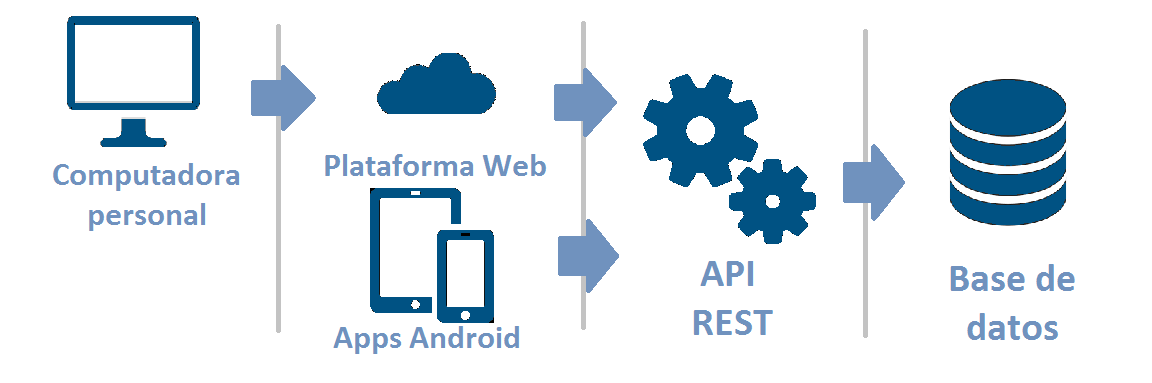
\includegraphics[scale = 0.7]{figures/proposedSystem}
	\caption{Diagrama propuesto del sistema.}
	\label{proposedSystem}
\end{figure}


\subsection*{Alcances}

El proyecto descrito en el presente documento se limita a la presentación cruda (no procesada o filtrada) de datos para el superusuario, en el registro de asistentes, miembros de staff, vendedores e inventarios para funcionar de manera integral, es decir, con interacciones entre todas las entidades descritas anteriormente.
Para el desarrollo de la API REST se utilizará el frameworkDjango REST cuya documentación y soporte se encuentran disponibles gratuitamente en línea, por lo que se evitará la generación de costos extraordinarios referentes al desarrollo de esta etapa del proyecto, pero limitando los alcances de ésta a los alcances del framework.

La API REST y la base de datos se almacenarán en servidores remotos gratuitos para evitar costos por desarrollo, despliegue, mantenimiento y consulta de ellos. Por lo tanto, el consumo de los servicios y la base de datos en sí, estarán limitados por las restricciones que conlleven dichos servidores gratuitos. Cabe aclarar que la plataforma será construida de manera escalable, y en el momento que sea requerido, estas dos entidades podrán ser trasladadas a plataformas con requerimientos y capacidades de mayor alcance.

\section{Objetivos}

		\subsection*{Objetivo general}
			Desarrollar una plataforma que permita el registro y administración de asistentes y vendedores en eventos de asistencia masiva que permitan la administración y consulta de cambios y transacciones mediante el acceso por medio de un sitio web y aplicaciones en el sistema operativo Android.
		\subsection*{Objetivos específicos}
		\begin{itemize}
			\item Diseñar e implementar una base de datos que permita el almacenamiento y fácil acceso a los datos importantes de perfil y transacciones de asistentes y vendedores.
			\item Desarrollar una API REST que permita el registro, actualización, consulta y eliminación de datos por medio de servicios.
			\item Desplegar un sitio web que permita la consulta de datos en tiempo real de las eventualidades ocurridas durante el curso del evento.
			\item Desarrollar una aplicación en Android para la administración de perfiles de asistentes.
			\item Desarrollar una aplicación en Android para control de acceso de asistentes.
			\item Desarrollar una aplicación en Android de punto de venta.
		\end{itemize}

\renewcommand{\thesection}{\arabic{section}} 
%\setcounter{section}{0}
\section{Estado del arte}\label{sec:stateoftheart}

\subsection{Proyectos internos del IPN}

\subsubsection*{Sistema NFC para cobro en una cafetería}

Se trata del diseño, construcción e implementación de un sistema que usa etiquetas NFC para identificar a los usuarios y miembros de personal de una cafetería, así como las interacciones entre ellos.

\subsubsection*{Diseño de una aplicación para inventarios utilizando tecnología NFC}

Se trata del diseño y desarrollo de una plataforma para controlar inventarios de productos a los que se debe incrustar una etiqueta NFC.

\subsubsection*{Control de acceso mediante NFC}

Se trata del diseño y desarrollo de una plataforma para garantizar o denegar el acceso a una zona a individuos identificados por una etiqueta NFC a las que se les pueden otorgar distintos permisos de acceso.

\subsection{Proyectos externos al IPN}

\subsubsection*{TopTap}

Plataforma de control de acceso, inventario y venta en eventos de asistencia masiva destinada a la administración por parte de grupos privados y desarrollado por la empresa POLIMENTES. El único evento hasta la fecha en el que dicha plataforma se ha desplegado fue el Bonfire Block Party de 2016, llevado a cabo en Colorado, E.U.

\subsubsection*{Intellitix}

Plataforma de inventario y venta en eventos de asistencia masiva destinada a la administración por parte del vendedor. Actualmente esta plataforma se encuentra disponible solamente en los Estados Unidos y su uso puede ser concedido previa negociación con la empresa desarrolladora.

\section{Marco teórico}

\subsection {Manejo de información personal}

Ya que la plataforma propuesta requerirá de un registro de usuarios para ligar a su boleto de acceso, se debe profundizar en el qué y cómo hacer una correcta manipulación de la información personal que resulte necesaria para el correcto funcionamiento de la plataforma.

El artículo 6 de la Ley Federal de Protección de Datos Personales en Posesión de los Particulares\cite{diarioOficial2010} dice “Los responsables en el tratamiento de datos personales, deberán observar los principios de licitud, consentimiento, información, calidad, finalidad, lealtad, proporcionalidad y responsabilidad, previstos en la Ley”. También cita en el índice III del artículo 10 que no será necesario el consentimiento para el tratamiento de los datos personales cuando los datos figuren en fuentes de acceso público.

Debido a que los únicos datos contemplados para el registro personal son el nombre, la edad y dirección de correo electrónico, todos ellos disponibles en fuentes de acceso público y obtenidos de manera clara y consensuada, no es necesaria la incorporación de ningún reglamento extraordinario para su manejo.

\subsection{API REST}

\subsubsection*{Concepto de API}

Una API es el mecanismo más útil para conectar dos softwares entre sí para el intercambio de mensajes o datos en formato estándar como XML o JSON. Así es como se convierte en un instrumento para buscar ingresos, abrirse al talento, innovar y automatizar procesos\cite{bancomer2016}.

Igual que una interfaz de usuario permite la interacción y comunicación entre un softwarey una persona, una API (acrónimo de Application Programming Interface) facilita la relación entre dos aplicaciones para el intercambio de mensajes o datos. Un conjunto de funciones y procedimientos que ofrece una biblioteca para que otro software la utilice como capa de abstracción, un espacio de acceso e intercambio de información adicional en la parte superior. Así una se sirve de la información de la otra sin dejar de ser independientes.

Cada API está diseñada en un lenguaje de programación concreto y con unas especificaciones distintas que la definen (las APIs pueden incluir especificaciones para estructuras de datos y rutinas, clases de objetos o
10variables, a partir de las cuales se basa el uso de esa interfaz). Además, suele ser habitual que cada una de ellas disponga de documentación completa y eficaz (un conjunto de tutoriales, manuales y reglas de buenas prácticas para esa interfaz de programación).

\subsubsection*{Tipos de API}

\begin{itemize}
  \item APIs de servicios web: son las interfaces de desarrollo de aplicaciones que permiten el intercambio de información entre un servicio web (software que da acceso a un servicio concreto a través de una URL) y una aplicación. Normalmente ese intercambio se produce a través de peticiones HTTP o HTTPS (la versión cifrada del protocolo HTTP). En la petición de la aplicación y respuesta, también en HTTP del servicio web, se contiene información de todo tipo tanto en los metadatos de la cabecera como en los del mensaje, normalmente en dos tipos de formatos muy usados: XML o JSON. Hay cuatro tipos de API de servicios web habituales entre los desarrolladores: SOAP (\textit{Simple Object Access Protocol}), un protocolo estándar de intercambio de información y datos en XML entre dos objetos; XML-RPC, un protocolo de llamada a procedimiento remoto que usa XML como formato de datos y llamadas HTTP como sistema de comunicación; JSON-RPC, mismo protocolo pero en formato JSON; y REST (\textit{Representational State Transfer}), arquitectura de software para sistemas hipermedia en la World Wide Web; una API REST usa el protocolo HTTP.
  \item APIs basadas en bibliotecas: este tipo de APIs son las que permiten que una aplicación importe una biblioteca de otro software para hacer el intercambio de información. Hoy en día gran parte de las bibliotecas que dan acceso a productos y servicios están diseñadas en JavaScript. Las APIs en JavaScript suelen ser un ejemplo ilustrativo de APIs basadas en bibliotecas, por ejemplo las que se utilizan dentro del mercado de la cartografía web (servicios como Google Maps, Leaflet, ArcGIS, CartoDB, MapBox o D3.js).
  \item APIs basadas en clases: este tipo de interfaces de desarrollo de aplicaciones permite la conexión con los datos en torno a las clases, como es habitual en programación orientada a objetos con Java. La API de Java usa clases abstractas para la creación de aplicaciones igual que cualquier programa desarrollado en este lenguaje. Esas clases proporcionan todo lo necesario para realizar todo tipo de funciones dentro
11de esas aplicaciones. La interfaz de desarrollo de Java se organiza en paquetes y cada uno de esos paquetes contiene a su vez un conjunto de clases relacionadas entre sí.
  \item APIs de funciones en sistemas operativos: los programas de software están continuamente interactuando con los sistemas operativos. Eso es una afirmación obvia. La realidad es que, en muchos casos, la forma en la que lo hacen es a través de APIs. Sistemas operativos como Windows disponen de APIs que permiten esa comunicación entre programas y el OS. Esta es la lista completa de API de Windows: interfaz de usuario, acceso y almacenamiento de datos, mensajería, gráficos y multimedia, diagnóstico de errores, etc.
  \item
  \item
\end{itemize}

\subsection{Especificación de requisitos de software}

En esta sección se presenta la Especificación de Requisitos de Software (ERS) para la aplicación móvil que forma parte del proyecto terminal “Sistema web y móvil para gestionar ventas y acceso en eventos de asistencia masiva utilizando etiquetas NFC” según el estándar de IEEE 830.

%\subsubsection{Propósito}

%El propósito de este documento es definir la estructura y diseño de la aplicación móvil. Este documento va dirigido a toda persona interesada en el funcionamiento y estructuración del software a desarrollar.

\subsubsection{Ámbito del software}

\begin{itemize}
\item	La aplicación móvil llevará por nombre “TapTop”.
\item	La aplicación interpretará un mensaje de voz a lenguaje de señas, representando el mensaje por medio de imágenes o animaciones.
\item	La aplicación no guardará los mensajes de voz.
\item	La aplicación contará con la capacidad de realizar síntesis de voz.
\item	No se podrán enviar mensajes digitales a través de la aplicación con otros usuarios.
\item	La aplicación permite la consulta de un diccionario del LSM por categorías.
\item	La aplicación reconocerá e interpretará cierta cantidad de frases limitadas por 43 palabras que se encuentran en el banco de reconocimiento.
\item	Con el desarrollo de esta aplicación se espera que las personas que utilizan el lenguaje de señas sean capaces de comunicarse con personas que no y a su vez, las personas que no hacen uso de éste sean capaces de comunicarse con personas que sí.
\item	Un beneficio de esta aplicación es que cualquier persona que cuente con un móvil Android podrá hacer uso de ella, sin hardware adicional.
\item	El objetivo de la aplicación móvil es lograr que las personas tengan mayor oportunidad de acercamiento a tecnologías que permitan realizar la comunicación sin hacer uso de hardware adicional.
\item	Se espera que el software en un futuro pueda ser capaz de admitir una ampliación a su vocabulario a reconocer.
\end{itemize}

\subsubsection{Del sistema}

\begin{itemize}
\item	La aplicación móvil tendrá conexión al servidor que llevará a cabo el procesamiento de voz y nos entregará el resultado, la conexión mediante Internet.
\item	El sistema permitirá el uso en cualquier momento.
\item	El sistema soportará diversas peticiones al mismo tiempo, el número de peticiones está por definirse de acuerdo a los algoritmos implementados.
\end{itemize}

\subsubsection{Visión general}

En las secciones siguientes se detalla la estructura y funcionamiento de la aplicación móvil, los requisitos del dispositivo que la ejecutará, diagramas de casos de uso, actividades y un esbozo general de la aplicación.

\subsubsection{Descripción general}
\paragraph{Perspectiva del producto}\paragraph{}

La aplicación móvil será totalmente independiente a cualquier otro producto, en un futuro la unión de dos aplicaciones no queda descartada, pues existen productos desarrollados y en desarrollo que contribuyen al proceso de comunicación con el uso del LSM y esta unión se podrá dar gracias a un content provider entre ambas aplicaciones. Para este trabajo se desarrollará la aplicación móvil que realice la traducción de un mensaje de voz a lenguaje de señas, se diseñará la aplicación móvil y desarrollará el sistema que permita el procesamiento de voz.

\paragraph{Funciones del producto}\paragraph{}

La aplicación móvil contará con tres funciones principales:

\begin{itemize}
\item	Traducción de voz a LSM: Esta función básicamente graba una frase en voz y la traduce a lenguaje de señas mexicana, mostrando el resultado mediante imágenes.
\item	Reproducción en voz de cualquier texto ingresado: Se toma el texto ingresado en un campo de texto y se realiza la síntesis en voz de éste.
\item	Consulta de un diccionario de LSM: Organizado por categorías, se podrán consultar palabras del LSM y la forma en que se realizan dichas señas.
\end{itemize}

\paragraph{Características de los usuarios}\paragraph{}

La aplicación móvil va dirigida a personas con interés de comunicarse principalmente con personas sordas que utilizan el LSM, además, también va dirigido a personas que utilizan el lenguaje de señas y que tienen interés en comunicarse con personas que no lo usan, estas personas deberán tener conocimiento básico del uso de aplicaciones móviles.

\paragraph{Restricciones y limitaciones}

El uso de esta aplicación se recomienda en dispositivos móviles con las siguientes características mínimas:
\begin{itemize}
\item	Smartphone Android versión 4.4.
\item	Memoria RAM de 1 GB.
\item	Memoria interna de 8 GB con memoria externa.
\item	CPU: Quad-core 1.4 GHz
\end{itemize}

Para el servidor que realizará el procesamiento:
\begin{itemize}
\item	Windows 8 o superior.
\item	Java 8 o superior.
\item	4 GB de memoria RAM.
\item	10 GB de disco duro disponibles.
\item	Procesador de doble núcleo a 1.8 GHz.
\item	MySQL server 5.6.
\end{itemize}

La aplicación será desarrollada en Android Studio versión 2.2 bajo el lenguaje de programación Java, el procesamiento de voz se llevará a cabo en un servidor con lenguaje C.

La comunicación con el servidor se llevará a cabo mediante web service a través del protocolo TCP/IP.

La aplicación móvil no contará con sistema de seguridad ya que no se estarán manejando datos delicados ni registro en ésta.

\paragraph{Suposiciones y dependencias}\paragraph{}

La aplicación móvil está diseñada para Android, si se desea migrar a otro sistema operativo se deberán revisar los requisitos del dispositivo, así como el cambio de desempeño e interfaces con el servidor, de igual forma, si el servidor se implementa en un sistema operativo, será necesario revisar la comunicación que se llevará a cabo con la aplicación móvil.

El número de palabras y/o frases en un futuro puede crecer, así que es posible que se requiera un servidor con mayor capacidad de procesamiento para llevar a cabo el reconocimiento de palabras.

\paragraph{Requisitos futuros}\paragraph{}

Las posibles mejoras a la aplicación serían la integración de un diccionario más amplio de reconocimiento, integración de un sistema de reconocimiento de imágenes para completar la comunicación bidireccional e incluir un curso sobre lenguaje de señas.

\subsubsection{Requisitos específicos}

\paragraph{Interfaces externas}

\begin{itemize}
\item	Ie1. La aplicación móvil tendrá una interfaz sencilla que permita al usuario intuir el funcionamiento y la sección de funciones de ésta.
\item	Ie2. La comunicación con el servidor se llevará a cabo mediante un web service a través del protocolo TCP-IP.
\item	Ie3. Para la realización de la función de \textit{text-to-speech} o síntesis de voz se hará uso de la API que Google nos proporciona.
\item	Ie4. El servidor utilizará el ODBC más adecuado  para comunicarse con la base de datos.
\end{itemize}

\paragraph{Funciones}
\begin{enumerate}[label=(\alph*)]
\item	Traductor de voz a LSM

\begin{itemize}
\item	Fa1. Se contará con un botón para iniciar la grabación de la voz. (Móvil)
\item	Fa2. Se enviará la voz o las características de ésta al servidor a través de un web service. (Móvil)
\item	Fa3. Se realizará el procesamiento de voz para determinar las palabras mencionadas. (Servidor)
\item	Fa4. Se mapeará la frase detectada con la estructura correspondiente al LSM. (Servidor)
\item	Fa5. Se leerá de la base de datos las imágenes o animaciones correspondientes a la frase detectada. (Servidor)
\item	Fa6. Se enviará a la aplicación móvil las imágenes o códigos de éstas para que en la pantalla muestre el mensaje con la estructura correcta. (Servidor)
\item	Fa7. La aplicación móvil mostrará en pantalla las imágenes o animaciones correspondientes a la frase mencionada.
\item	Fa8. El usuario sólo podrá decir frases cortas con duración no mayor a 10 segundos.
\end{itemize}

\item	Síntesis de voz a través del teclado

\begin{itemize}
\item	Fb1. El usuario a través del teclado en pantalla ingresa la frase a comunicar.
\item	Fb2. Haciendo uso de la API de Google de text to speech se realizará la síntesis del texto introducido.
\item	Fb3. El idioma soportado será el español de México.
\end{itemize}

\item	Diccionario del LSM

\begin{itemize}
\item	Fc1. El diccionario estará dividido por categorías.
\item	Fc2. Contará con filtros por categoría y un cuadro de búsqueda.
\item	Fc3. Al seleccionar la palabra, la aplicación le mostrará la imagen correspondiente, además de una breve descripción de su uso.
\end{itemize}

\end{enumerate}

Estas secciones serán alcanzables gracias a un menú lateral que nos ofrecerá la opción de ingresar a cada una.

\paragraph{Requisitos de rendimiento}
\begin{itemize}
\item	Rr1. La aplicación sólo podrá ejecutar una actividad a la vez, y será usada por un usuario.
\item	Rr2. La aplicación se conectará con el servidor que ejecutará el procesamiento de la voz.
\item	Rr3. El servidor tendrá la capacidad de atender a más de un usuario a la vez .
\item	Rr4. Se requiere que la aplicación cuente con conexión a Internet.
\item	Rr5. Dado el listado de palabras se plantea que la cantidad de registros almacenados en la base de datos sea en el orden de las decenas.
\end{itemize}

\paragraph{Restricciones de diseño}
\begin{itemize}
\item	Rd1. La interfaz de la aplicación móvil se desarrollará en Android Studio, haciendo uso de las formas ya establecidas.
\item	Rd2. La interfaz gráfica de la aplicación móvil se llevará a cabo siguiendo el diseño visual y de movimientos de la guía de Material Design para Android.
\item	Rd3. La interfaz será de fácil entendimiento para que todas las personas que lo deseen la puedan ocupar.
\item	Rd4. El servidor no contará con interfaz gráfica.
\item	Rd5. Se hará uso del diccionario “manos con voz” de María Serafín y Raúl González para la obtención de imágenes.
\end{itemize}

\paragraph{Atributos de la aplicación}
\begin{itemize}
\item	Aa1. La aplicación será diseñada para que pueda ser usada por todo tipo de personas.
\item	Aa2. No se requiere de un inicio de sesión, por lo que en un móvil pueden interactuar más personas.
\item	Aa3. Como trabajo a futuro serán ofrecidas las actualizaciones que permitan más características, así como también nuevas funciones.
\end{itemize}

\include{./sections/design}
\include{./sections/conclusions}
\include{./sections/acronymList}

\newpage
\bibliographystyle{ieeetr}
\renewcommand{\bibname}{Bibliography}
\bibliography{./ref/references}

\end{document}